\documentclass[border=5pt]{standalone}
\usepackage{tikz}
\usepackage{amsmath}
\begin{document}
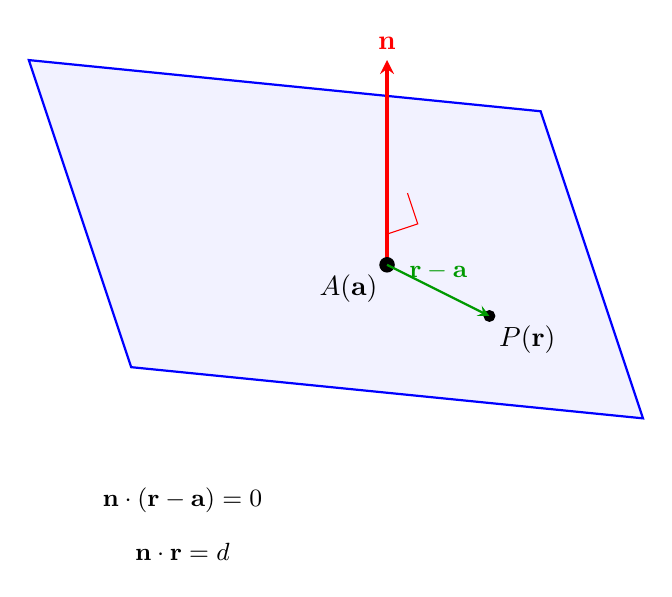
\begin{tikzpicture}[scale=1.3, >=stealth]
  % Plane with normal vector

  % Plane (parallelogram in perspective)
  \fill[blue!10, opacity=0.5] (-2,0.5) -- (3,0) -- (2,3) -- (-3,3.5) -- cycle;
  \draw[thick, blue] (-2,0.5) -- (3,0) -- (2,3) -- (-3,3.5) -- cycle;

  % Normal vector n (perpendicular to plane)
  \draw[->, very thick, red] (0.5, 1.5) -- (0.5, 3.5) node[above] {$\mathbf{n}$};

  % Right angle symbol
  \draw[red, thin] (0.5, 1.8) -- (0.8, 1.9) -- (0.7, 2.2);

  % Point A on plane
  \filldraw[black] (0.5, 1.5) circle (2pt) node[below left] {$A(\mathbf{a})$};

  % General point P on plane
  \filldraw[black] (1.5, 1.0) circle (1.5pt) node[below right] {$P(\mathbf{r})$};

  % Vector from A to P
  \draw[->, thick, green!60!black] (0.5, 1.5) -- (1.5, 1.0) node[midway, above, font=\small] {$\mathbf{r}-\mathbf{a}$};

  % Equation labels
  \node[font=\small] at (-1.5, -0.8) {$\mathbf{n}\cdot(\mathbf{r}-\mathbf{a}) = 0$};
  \node[font=\small] at (-1.5, -1.3) {$\mathbf{n}\cdot\mathbf{r} = d$};
\end{tikzpicture}
\end{document}
